\documentclass[11pt]{book}

\usepackage{graphicx}
\usepackage[dvipsnames]{color}
\usepackage[hidelinks]{hyperref}
\usepackage[square,numbers]{natbib}
\bibliographystyle{abbrvnat}
%pPara poder modificar los margenes
\usepackage{vmargin}
%Para usar el español
\usepackage[spanish]{babel}
\usepackage[utf8]{inputenc}
\usepackage{hyperref}
\begin{document}
%Portada
\setpapersize{A4}


%Indice

\tableofcontents
\newpage
\listoffigures
\chapter*{Resumen} 
Un proyecto ApS es una practica académica que combina procesos de aprendizaje y servicio a la comunidad para ayudar al alumnado a implicarse en proyectos y actividades de su entorno. De esta manera el alumnado podrá adquirir nuevos conocimientos y progresar en su desarrollo de aprendizaje en la universidad.\\\\
Este \textit{Trabajo de Fin de Grado} (TFG) es la continuación de un TFG titulado \textit{Desarrollo de una comunidad web para el soporte virtual del Aprendizaje-Servicio III}, realizado por David Jimenez Del Rey en la \emph{Universidad Nacional de Educación a Distancia} (UNED). Su TFG fue dirigido por Ángeles Manjarrés y codirigido por Simon Pickin. \\\\
Los profesores con experiencia en iniciativas de tipo ApS se dieron cuenta de que un buen soporte informático podría ser de gran ayuda en la difícil tarea de casar la oferta y la demanda de ApS. Gracias a este soporte se facilitarían la identificación de potenciales partenariados así como la colaboración entre el prestador y el receptor potenciales del servicio en la tarea de refinar una idea inicial y convertirla en un propuesta de proyecto realista que cumple las necesidades de las dos partes.\\\\ 
Partiendo del TFG de David Jimenez Del Rey, los objetivos de nuestro \textit{Trabajo de Fin de Grado} fueron crear un modelo de dominio, un modelo de datos y un modelo relacional para la aplicación, cambiar de una base de datos no relacional, MongoDB, a una base de datos relacional, MySQL, implementar \emph{Objetos de Acceso a Datos}(DAOs) para encapsular el acceso a la base de datos, crear \emph{Objetos de Transferencia de Datos} (DTOs) para el transporte de los datos entre las diferentes capas de la aplicación, implementar un sistema de \textit{matching} entre las ofertas de los profesores y las demandas de los socios comunitarios, adaptación del código de los formularios ya creados en el anterior proyecto,tales como registro  y editar perfil de usuarios y la implementación de unos nuevos para la creación  de la oferta, la demanda y los partenariados y la corrección del TFG precedente.\\\\
Nuestro TFG fue desarrollado usando tecnologías como Angular, Express, JavaScript, Node.js y MySQL, donde la mayoría de estas tecnologías ya se habían usado en el anterior TFG.\\\\
\addcontentsline{toc}{chapter}{Resumen} 
\markboth{RESUMEN}{RESUMEN} 
\chapter*{Abstract} 
An ApS project is an academic practice that combines learning processes and community service to help students get involved in projects and activities in their environment. In this way, students will be able to acquire new knowledge and progress in their learning development at university. \\\\
This \textit{Final Degree Project} (TFG) is the continuation of a TFG titled \textit{Development of a web community for the virtual support of Service-Learning III}, carried out by David Jimenez Del Rey at \emph{National University of Distance Education} (UNED). His TFG was directed by Ángeles Manjarrés and co-directed by Simon Pickin. \\\\
Teachers with experience in ApS initiatives realized that good IT support could be of great help in the difficult task of matching the supply and demand of Aps. Thanks to this support, the identification of potential partnerships would be facilitated as well as the collaboration between the provider and the potential recipient of the service in the task of refining an initial idea and turning it into a realistic project proposal that meets the needs of both parties. \ \\\
Based on David Jimenez Del Rey's TFG, the objectives of our \ textit {Final Degree Project} were to create a domain model, a data model and a relational model for the application, change from a non-relational database, MongoDB, to a relational database, MySQL, implement \ emph {Data Access Objects} (DAOs) to encapsulate access to the database, create \ emph {Data Transfer Objects} (DTOs) for transport of the data between the different layers of the application, implement a system of \ textit {matching} between the offers of the teachers and the demands of the community partners, adaptation of the code of the forms already created in the previous project, such as registration and edit user profiles and the implementation of new ones for the creation of supply, demand and partnerships and the correction of the previous TFG. \\\\
Our TFG was developed using technologies such as Angular, Express, JavaScript, Node.js and MySQL, where most of these technologies had already been used in the previous TFG.\\\\
\addcontentsline{toc}{chapter}{Abstract} 
\markboth{Abstract}{Abstract} 

\chapter{Matching entre oferta de servicio y demanda de servicio}\label{cap:matching}

\section{Definición del matching }

Para nuestro TFG hemos implementado un algoritmo de \emph{matching} para las ofertas y las demandas, de manera que cogiendo una oferta y una demanda de la base de datos, verificamos si tienen suficientes similitudes como para poder establecer un partenariado a partir de ellas. Partiendo de unas especificaciones del algoritmo que se estableció entre nosotros y los directores del TFG, las hemos aplicado para poder obtener la información relacionada representada por un porcentaje, con el cual se decidirá el resultado final.  Cuantos más datos haya relacionados entre una oferta y una demanda, mayor porcentaje sacará nuestro algoritmo. El objetivo del algoritmo de \emph{matching} es ayudar a los profesores a encontrar más fácilmente demandas relacionadas a sus propuestas y a las entidades a obtener ofertas acordes a sus solicitudes. \\\\
El problema de \emph{matching} en el contexto de proyectos ApS conlleva varias dificultades. Entre ellas, la ausencia de una simetría entre la información proporcionada entre las ofertas y demandas. Esto no ocurre en aplicaciones de otra naturaleza como, por ejemplo, las aplicaciones de búsqueda de alquileres de pisos. Un posible usuario puede demandar un piso que, por ejemplo, tenga tres habitaciones y esté situado en el centro, mientras que otro usuario distinto puede ofertar en alquiler un piso con esas mismas características, por lo que el match sería evidente en este caso. Esto se debe a que tanto las ofertas como las demandas de alquiler tienen el mismo tipo de información, lo que las hace fácilmente contrastables. Sin embargo, en el marco de un proyecto ApS esto no es así. Las ofertas suelen ser más genéricas, y las demandas son más específicas, por lo que no existe simetría total entre los campos de ambas entidades.\\\\
Definimos el \emph{matching} según nuestro algoritmo, como el proceso que consiste en identificar los datos que se ajustan a unos criterios de coincidencia los cuales se van a enumerar a continuación en los siguientes párrafos. De este modo, si se encuentran suficientes puntos de similitud entre los datos recopilados, estos son considerados para sacar un porcentaje de coincidencia, donde si este es menor que el valor mínimo establecido no se considerará \emph{matching}. En el prototipo que hemos construido, el valor mínimo que hemos
establecido para considerar la existencia de un \emph{matching} es \texttt{50\%} pero, al
igual que los pesos de cada factor, es configurable.
\\\\

\section{Criterios de matching y anti matching}
\subsection{Criterios de matching }

Hemos definido unos criterios en base a los datos proporcionados por los usuarios en las ofertas y demandas de servicio según los cuales se resolverá el \emph{matching}:

\begin{itemize} 	
	\item Hacer coincidir las descripciones tanto de la oferta como de la demanda de servicio mediante Procesamiento del Lenguaje Natural (NLP).
	Para ello hemos tenido que buscar las palabras vacías del idioma español y almacenarlas en un fichero, para así poder  procesarlas para obtener el resultado deseado. El procedimiento consiste en lo siguiente: dadas las dos descripciones, las guardamos en dos estructuras simples de datos, quitamos las palabras comunes (aquellas que sean iguales a las del fichero) y nos quedamos con las que puedan coincidir en las dos descripciones. Cada una de estas se guarda en una estructura simple de datos. Al tenerlas, empezamos a procesar las palabras resultantes de las dos descripciones, distinguiendo las mayúsculas, minúsculas, tildes y caracteres especiales, donde obtenemos el número de palabras que coinciden de las descripciones. Para poder obtener el porcentaje de coincidencias, dividimos el número de palabras coincidentes con el número de palabras de la descripción mas breve. Dicho porcentaje se tendrá en cuenta para poder calcular el valor final de \emph{matching}.
	
	\item Encontrar la similitud entre las áreas de implementación tanto de la oferta como de la demanda. Hemos poblado la base de datos con setenta y ocho áreas de implementación para poder realizar esta comprobación. Para ello se comparan todas las áreas de implementación de ambas, y se devuelve el número de coincidencias. Cuanto mayor dicho número, mayor probabilidad de que se produzca el \emph{matching}.
	
	\item Obtener las coincidencias entre las titulaciones que el socio
	comunitario ha propuesto como candidatos en los que cuadrar un proyecto
	ApS a la hora de introducir la demanda (si es que ha introducido algunas) con las titulaciones en las que imparten docencia los profesores asociados a la oferta. 
	Hemos poblado la base de datos del prototipo con ciento nueve titulaciones locales para poder realizar esta comprobación. Tanto la oferta como la demanda pueden tener una o varias titulaciones, y en función de la cantidad de titulaciones de la demanda, se calcula el resultado, el cual será un porcentaje obtenido a partir de la división del número total de titulaciones que producen coincidencias entre el  número total de las titulaciones de la demanda. Este campo es opcional, y en el caso de que no este relleno no se va a proceder dicha comprobación.
	
	\item Obtener las coincidencias en las observaciones temporales de la oferta de servicio y de la demanda de servicio para las que hemos aplicado Procesamiento del Lenguaje Natural (NLP). Una vez obtenidas las dos observaciones temporales, tanto de la oferta como de la demanda, procedemos a aplicar el algoritmo para emparejar las palabras que coinciden en ambos lados y obtener un porcentaje. Para ello una vez más se quitan las palabras comunes de las descripciones y se guardan las palabras no comunes para cada una de las observaciones temporales en una estructura de datos. Tras esto, se procesan cada una de las estructuras, resultando el número de observaciones temporales que coinciden. El porcentaje de coincidencias se obtiene mediante la división del número de palabras coincidentes entre el valor (observaciones temporales) que tiene el menor número de palabras.
	
	\item Relacionar el área de implementación de la demanda con las titulaciones en las que imparten docencia los profesores que participan en la oferta. Para ello tenemos asignados al menos una titulación a cada área de implementación. Estas relaciones están almacenadas en una tabla de la base de datos. De esta manera se podrá obtener la relación directa o indirecta entre estos dos valores para así poder calcular un porcentaje válido para el resultado final de nuestro algoritmo de \emph{matching}. Por ejemplo el área de implementación \texttt{Computer\_science} se relacionaría con las titulaciones \emph{Ingeniería de Computadores}, \emph{Ingeniería Informática}", \emph{Ingeniería del Software}, \emph{Telecomunicación}, etc. Para el cálculo del porcentaje se usa el mismo procedimiento que en los demás criterios: contamos el número de coincidencias y lo dividimos entre la cantidad total de las áreas de implementación.
	
	\item Encontrar la similitud entre el área de implementación de la demanda y las áreas de conocimiento UNESCO de los profesores que participan en la oferta. Para ello tenemos asignados al menos un área de conocimiento a cada área de implementación. Estas relaciones están almacenadas en la tabla \texttt{matching\_areas} de la base de datos. Se dispone de ciento noventa áreas de conocimiento en la base de datos para poder realizar esta comprobación. Para ello tenemos en cuenta las áreas de conocimiento con las cuales están relacionadas las áreas de implementación de la demanda y de la oferta como el principal valor en el cálculo del porcentaje. Para encontrar las posibles coincidencias contamos el número de ellas y lo dividimos entre el número de áreas de implementación de la demanda.
\end{itemize}

	Para un futuro proyecto, se debería implementar la obtención de las coincidencias entre las
	titulaciones que el socio comunitario ha propuesto como posibles y las
	titulaciones a las que pertenecen las asignatura/s identificadas en la
	oferta como asignatura/s objetivo. 

\subsection{Criterios de anti matching }

También hemos definido unos criterios de \emph{anti matching} para encontrar posibles incompatibilidades entre los datos proporcionados.\\\\
Para poder realizar el \emph{anti matching} nos hemos centrado en los valores temporales, en el caso de que tengan valor puesto, tanto de la demanda como de la oferta. Para ello hemos partido de si el comienzo del periodo de disponibilidad para trabajar en la definición
de un proyecto ApS definido por la demanda no es posterior a la fecha límite para terminar la
definición del proyecto definida por la oferta. En el caso de que esté fuera del plazo se considera \emph{anti matching} y se descartará la posibilidad de una negociación entre dicha demanda y oferta. \\\\

En el caso de que los plazos estén en el periodo aceptado, se procede a
verificar si alguno de los siguientes se cumple 
\footnote{donde
	\begin{itemize}
		\item si la demanda define un periodo de disponibilidad para trabajar
		en la realización del proyecto ApS, denotamos con
		$\mbox{comienzo}\_\mbox{dispR}$ y $\mbox{fin}\_\mbox{dispR}$ las fechas
		del comienzo y del fin de este periodo,
		\item si la oferta define un año académico en el que realizar el
		proyecto, denotamos con $\mbox{comienzo}\_\mbox{Año}$ y
		$\mbox{fin}\_\mbox{Año}$ las fechas del comienzo y del fin de este año
		académico,
		\item si la oferta define un cuatrimestre en el que realizar el
		proyecto, además de definir un año académico, denotamos con
	 	$\mbox{comienzo}\_\mbox{Cuat}$ y $\mbox{fin}\_\mbox{Cuat}$ las fechas del
		comienzo y del fin de este cuatrimestre de este año académico
	\end{itemize} }:

\begin{itemize}
	\item Si la demanda define un periodo de disponibilidad para la
	realización y la oferta define un año académico y
	$\mbox{fin}\_\mbox{dispR} < \mbox{comienzo}\_\mbox{Año}$
	o
	$\mbox{comienzo}\_\mbox{dispR} > \mbox{fin}\_\mbox{Año}$
	\begin{itemize}
		\item Si, al contrario,
		$\mbox{fin}\_\mbox{dispR} \geq \mbox{comienzo}\_\mbox{Año}$
		o
		$\mbox{comienzo}\_\mbox{dispR} \leq \mbox{fin}\_\mbox{Año}$,
		pero la oferta también define un cuatrimestre y
		$\mbox{fin}\_\mbox{dispR} < \mbox{comienzo}\_\mbox{Cuat}$
		o
		$\mbox{comienzo}\_\mbox{dispR} > \mbox{fin}\_\mbox{Cuat}$.
	\end{itemize}
\end{itemize}
 Si no se cumple alguna de estas condiciones, se considera \emph{anti matching} y en caso contrario se continúa con la comprobación de los siguientes valores temporales.\\\\

Otro criterio de \emph{anti matching} es comprobar si la fecha límite para el fin de la realización del proyecto ApS definido por la demanda es menor que la fecha de inicio del cuatrimestre en el año académico elegido de la oferta. De modo, si no se corresponden correctamente, se considera incompatibilidad y se descarta la negociación. \\\\



\section{Obtención del porcentaje final de matching}

Una vez obtenidos todos los porcentajes de los criterios de \emph{matching} y los resultados del \emph{anti matching} procedemos a combinar todos los criterios en un único porcentaje. Para ello multiplicamos cada uno de los porcentajes anteriormente mencionados por los pesos que les corresponden a cada uno definidos en el fichero \texttt{configuracion.txt} y son sumados para obtener el valor de compatibilidad entre la oferta y la demanda. El fichero \texttt{configuracion.txt} almacena en cada línea datos como \texttt{pesoFechas = 0.3}, \texttt{pesoTitulaciones = 0.3}, \texttt{pesoAreaServicio = 0.2}...  \\\\

Si el valor obtenido es mayor que 0.5, valor que es configurable, se considerará un match definitivo y se almacenará en la base de datos en un tabla que contendrá el porcentaje final, el identificador de la oferta, el identificador de la demanda y un atributo booleano, \emph{procesado}, que se pone a true indicando si paso por el proceso de verificación del match. 
El atributo \emph{procesado} sirve para evitar repetir comparaciones entre ofertas y demandas. En el caso de que una demanda y una oferta no pasaron por el algoritmo de \emph{matching}, este atributo \emph{procesado} tendrá el valor a false. Si una oferta y una demanda pasaron por el proceso de verificación de \emph{matching} tendrán guardados en la tabla el porcentaje de \emph{matching}, que puede ser superior, inferior o igual a 0.5, y el valor del atributo \emph{procesado} a true. La tabla de \texttt{matching} de la base de datos contendrá la información sobre los posibles \emph{match} y \emph{no match} de entre las demandas y ofertas procesadas, de esta manera la aplicación del algoritmo de \emph{matching} se ejecuta una única vez por cada pareja oferta-demanda. \\\\

A partir de un \emph{matching} de una oferta de servicio y una demanda se crea un partenariado en el caso de que el profesor quiera. Para ello, primero, el profesor responsable de la oferta acepta el match y rellena el formulario que tiene  algunos campos rellenados automáticamente a partir de información contenida en la oferta o en la demanda, lo que conlleva la creación de un partenariado en estado \texttt{EN\_CREACION} y el envío de una notificación a la socio comunitario. Después, el socio comunitario podría aceptar el \emph{match}, rellenando un segundo formulario, teniendo algunos campos rellenados automáticamente a partir de información contenida en la oferta o en la demanda, lo que provocaría que el partenariado pasará al estado \texttt{EN\_NEGOCIACION}.\\\\

\section{Ejemplo de matching}

A continuación se muestra un ejemplo válido de \emph{matching} con una oferta y una demanda dada, con un porcentaje de \emph{match} mayor del 50\%. Se expondrá la aplicación de cada uno de los criterios de \emph{matching} y \emph{anti matching}, y cómo se llegó al resultado final del algoritmo, de modo que se irá paso a paso por cada etapa del algoritmo que hemos creado.\\\\
Dada una oferta con los datos más significativos para el \emph{matching}:\\
\begin{itemize} 
	\item Descripción: Proyecto de investigación en biología y tecnología
	\item Observaciones temporales: Me interesa que se empiece en septiembre
	\item Área de implementación: Biología, Tecnología digital
	\item Área conocimiento: Biología celular
	\item Titulaciones: Grado en Ciencias Ambientales
	\item cuatrimestre objetivo: Primer cuatrimestre
	\item Fecha límite para terminar la definición del proyecto: 2021/12/22
	\\
\end{itemize}
Y una demanda con los datos:\\
\begin{itemize} 
	\item Titulaciones: Grado en Ciencias Ambientales
	\item Descripción: Proyecto de investigación en biología
	\item Observaciones temporales : En septiembre 2021
	\item Área de implementación: Biología
	\item Comienzo del periodo de disponibilidad para trabajar en la definición del
	proyecto : 2021/09/04
	\item Fin del periodo de disponibilidad para trabajar en la definición del
	proyecto: 2021/09/07
	\item Inicio del periodo de disponibilidad para trabajar en la realización del
	proyecto: 2021/09/14
	\item Fin del periodo de disponibilidad para trabajar en la realización del
	proyecto : 2021/12/01
	\item Fecha límite para el fin de la realización del proyecto: 2021/12/04
\end{itemize}
Se empieza comparando las fechas para detectar un posible \emph{anti matching}. En el ejemplo las fechas cuadran, así que multiplicamos el peso de este atributo que es 0.3. Después de esto se comprueban las titulaciones del profesor que hace la oferta, con las que podría tener la demanda. Como coinciden totalmente se multiplica el peso de este atributo por 0.3 y de momento hay un 0.6 de compatibilidad entre la oferta y la demanda. Tras esto se comprueban las áreas de implementación junto con las áreas de conocimiento de los profesores y se multiplica el porcentaje de coincidencias por el peso de este atributo, que es 0.2. Y actualmente hay una compatibilidad de 0.66. Tras esto empezamos a buscar las coincidencias mediante NLP entre las dos descripciones, quitamos las palabras comunes de ambas y nos quedamos con las no comunes. La descripción de la oferta se queda en “Proyecto,investigacion,biologia,tecnologia” y la de la demanda se queda en “proyecto,investigacion,biologia”. Obtenemos el porcentaje resultante entre el número de coincidencias que es tres y la longitud total de la descripción con menos valores, que es tres, por lo que se consigue el máximo de coincidencias entre las dos descripciones. Se obtiene el porcentaje de similitud entre 0 y 100,  en este caso es 0.60 y esto lo multiplicamos por 0.1 con lo que la compatibilidad actual seria 0.73. El mismo procedimiento se aplica también para las observaciones temporales, donde el número de coincidencias resultante es uno y el total de valores de la menor de las observaciones temporales es dos, por lo que el resultado tras ello es 0.33 de coincidencias, que se multiplica por 0.1 con lo que la compatibilidad actual seria 0.7366. La compatibilidad actual es de 0.74 y dado que es mayor que 0.5, se considera que la oferta y demanda encajan.\\\\
 Como se puede observar, tras el número elevado de coincidencias, se produce el \emph{matching} entre la oferta y la demanda y por lo consecuente se inserta la relación en la tabla \texttt{matching}.\\\\
 
 \chapter{Creación de formularios}\label{cap:formularios}
 Una vez adaptada la base de datos de no relacional a relacional y creados los correspondientes operaciones CRUD de las tablas, hemos pasado a la creación o a la adaptación de los formularios con los nuevos datos que les corresponde a cada uno de ellos. Para ello, tuvimos que aprender y experimentar con Angular, \emph{framework} de Javascript, que requiere un vasto conocimiento para el desarrollo de los formularios y de los archivos para el correcto funcionamiento de estos.
 \section{Formulario de registro de usuarios}
 El primer formulario que tuvimos que tratar fue el registro de usuarios, siendo este el punto de inicio para los posteriores formularios a crear.\\\\
 En la aplicación de la que partimos ya venía un registro implementado con sus correspondientes campos, pero al probar la aplicación habíamos encontrado algunos errores que tuvimos que corregir. Uno de los errores que encontramos era que el formulario permitía introducir una contraseña no robusta de cualquier longitud y sin ninguna restricción. De manera que la hemos hecho más robusta con una longitud mínima de 8 caracteres, mínimo una mayúscula, mínimo una minúscula y mínimo un carácter especial. Por otro lado, no se verificaba si el campo \emph{email} era correcto de modo que tuvimos que crear las validaciones correspondientes por si el valor introducido no contenía el signo \emph{@} o el signo \emph{(.)} .\\\\
 En el formulario de David Jiménez existían dos campos para la contraseña: \emph{contraseña} y   \emph{repetir contraseña}, donde ambos campos deben contener el mismo contenido para que se pueda permitir la validación del formulario y la creación del usuario. En cambio, si las contraseñas no coincidían lo aceptaba y se procedía al proceso de registro. Por eso tuvimos que añadir la validación y los mensajes de error correspondientes para que no se permita el registro si los dos campos no son iguales.\\\\
 Una vez arreglados los errores, añadidas las mejoras y las nuevas validaciones del registro tuvimos que añadir los campos nuevos correspondientes a cada tipo de usuario de la base de datos. \\\\
 En el formulario el \emph{email} del usuario sirve como atributo único, de manera que, si un usuario intenta registrarse con un email que ya esta en uso no se permitirá registrarse, llegando un mensaje de la aplicación de que el email ya esta en uso por otro usuario. \\\\
 En el formulario de registro se permite la elección de cuatro tipos de usuarios externos: profesor externo, estudiante externo, entidad y socios comunitarios. No están implementados el registro de los perfiles de colaboradores y Tutores de Centros Asociados de la UNED, donde deberían implementarse en un proyecto futuro. Ademas, se ha introducido en el formulario un nuevo campo \emph{teléfono} que sirve para todos los tipos de usuarios. A la hora registrarse los usuarios tendrán que dar el número de teléfono para ayudar con la autenticación manual.\\\\
 Para el socio comunitario aparte de los campos ya existentes en el formulario se añadieron los campos \emph{nombre socio comunitario} que representa el nombre del socio comunitario
 principal que creará el formulario, la \emph{URL} que representa la página web del socio comunitario y la \emph{misión} que representa la auto-descripción del registrante. \\\\
 En el caso del estudiante externo no se han añadido nuevos campos en el formulario, pero sí el cambio de funcionalidad del campo \emph{universidad}. Antes, en el campo \emph{universidad} se permitía introducir un texto, pero se convirtió en un menú desplegable que permite una única selección por el estudiante de entre ochenta y tres universidades a elegir de España. No se permite la validación del registro si no se selecciona alguna universidad de la lista. En un futuro se debería añadir un campo de texto \emph{universidad extranjera} que sea mutuamente exclusivo con el menú desplegable para que puedan participar profesores y alumnos de universidades extranjeras. Cuando un usuario va a elegir una universidad del menú desplegable, se bloqueará el campo de texto \emph{universidad extranjera}, y si el usuario escribirá algo en el campo de texto, se bloqueará el menú desplegable. \\\\
 Para el formulario del profesor externo se añadió un campo nuevo y se cambiaron las funcionalidades de algunos otros campos. El campo \emph{universidad} tenía el mismo problema que en el caso anterior por lo que se produjo el mismo cambio. Además, tuvimos que introducir un nuevo campo \emph{Área/s de conocimiento UNESCO}, que representa las áreas de conocimiento UNESCO que tiene el profesor externo a registrar. Este campo es un menú desplegable que permite la selección múltiple de entre las ciento noventa áreas disponibles que guardamos en la base de datos en la tabla \texttt{area\_conocimiento}. Se puede seleccionar entre una o varias áreas de conocimiento y en el caso de que se haya cometido un error al seleccionar un área se permite desmarcar la elección, pero no se permite la validación del registro en el caso de que no se haya seleccionado ningún área de conocimiento de la lista.\\\\
 Para que la aplicación pueda tener seguridad, en un futuro debería haber algún tipo de \emph{Captcha} para que se eliminen a los \emph{bots}. Ademas, existe en el formulario de registro un campo de texto para la misión del registrante, donde la Oficina ApS será la encargada de dar el visto bueno a esta petición de registro después de hacer las comprobaciones pertinentes. La Oficina ApS tendría la posibilidad de seleccionar las peticiones de registro de los socios comunitarios pendientes y tratarlas al entrar en la aplicación. Otra opción a la alternativa de la intervención humana seria permitir el uso del SSO de Google, de Microsoft, de Facebook, etc., pero como no se puede exigir a que los usuarios que quieran participar tener una cuenta en Google, Facebook, etc., esta opción no encaja con una aplicación destinada al sector público y al tercer sector. \\\\
 Aunque la figura \ref{fig:registro} contiene información especifica de la UNED, en un futuro esto será aplicable a cuentas universitarias pertenecientes a la universidad en la que está o la que esté desplegada la aplicación.
 
 
 \begin{figure}[t]
 	\centering
 	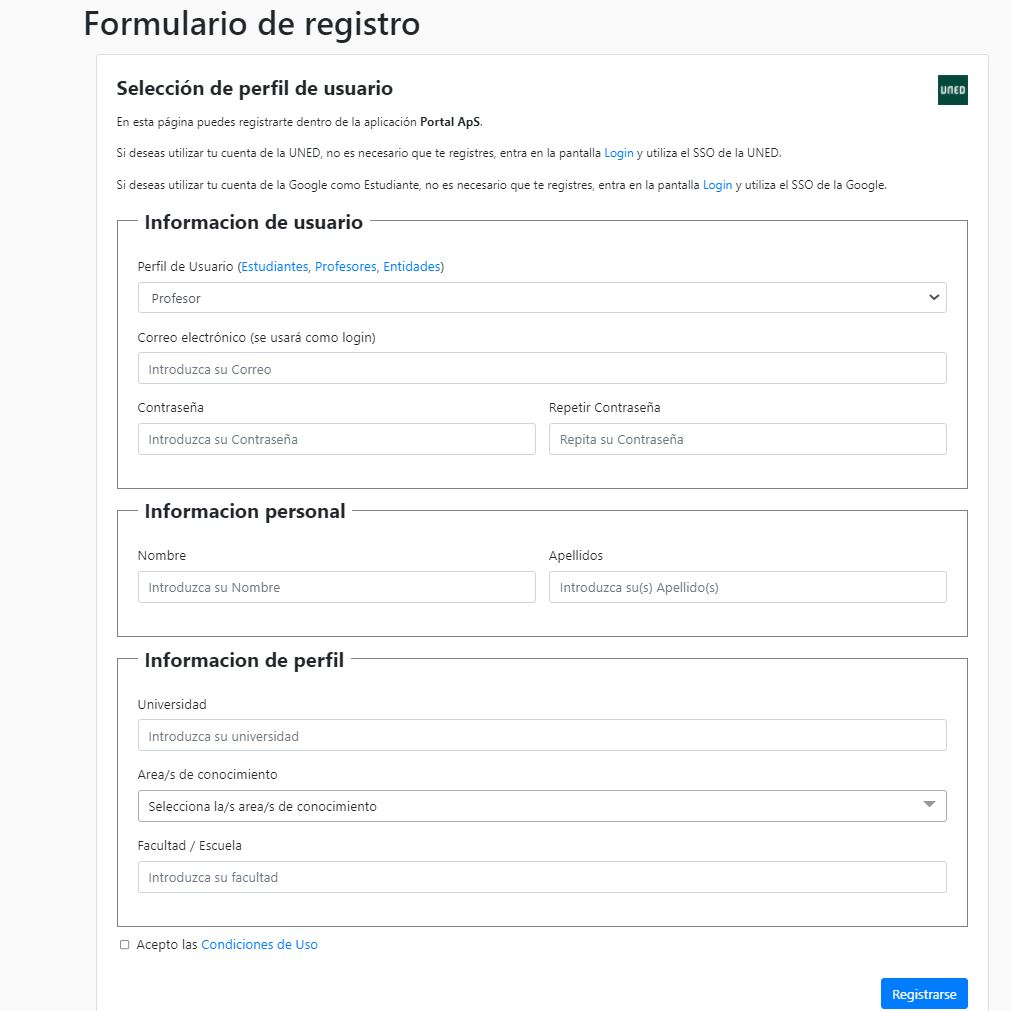
\includegraphics[scale=0.7]{registro}
 	\caption{Formulario de registro}
 \end{figure}
 
 \section{Formulario para editar los datos de un usuario}
 En el TFG de David Jiménez ya existía un formulario para la edición de los datos de un usuario con sus correspondientes campos, pero al cambiar el tipo de base de datos y al introducir nuevos datos en algunos de los tipos de usuarios tuvimos que adaptar este formulario. \\\\
 También añadimos las validaciones para los campos \emph{email}, \emph{contraseña} y \emph{repetir contraseña} como en el anterior formulario. Una vez añadidas las validaciones se introdujeron los campos necesarios para el formulario en función del tipo de usuario.\\\\
 Para el socio comunitario, aparte de los campos ya existentes en el formulario, se añadieron los campos \emph{nombre socio comunitario}, \emph{URL} y \emph{misión}. Los campos \emph{sector}, \emph{nombre socio comunitario}, \emph{URL} y \emph{misión} vienen con el valor ya rellenado, y no tienen la posibilidad de cambiar su valor. \\\\
 Para el estudiante externo no se han añadido nuevos campos en el formulario, pero sí el cambio de funcionalidad del campo \emph{universidad}, que se convirtió en un desplegable que permite una única selección por el estudiante.  No se permite la validación de registro si no se selecciona alguna universidad de la lista. El campo viene con el valor ya relleno, teniendo la posibilidad de cambiar su valor.\\\\
 En el caso del profesor externo el campo \emph{universidad} pasó a ser un campo que no se puede cambiar su valor debido a que, si cambia de universidad, inevitablemente cambiará también de dirección de mail corporativo. Además, tuvimos que introducir un nuevo campo \emph{Área/s de conocimiento UNESCO} que representa las áreas de conocimiento de un profesor. Se puede seleccionar al menos un área de conocimiento y el valor viene ya relleno con los valores del usuario ya creado.
 
 
 
 \section{Formulario creación demanda de servicio}
 Para poder crear una demanda de servicio en la base de datos tuvimos que crear el formulario desde cero con sus correspondientes archivos, puesto que en el anterior TFG no existía. Para ello se tuvo que crear su correspondiente modelo con los campos necesarios para la creación de la demanda: identificador, titulo, descripción, imagen, localización del servicio, objetivo, área de implementación, comienzo del periodo de disponibilidad para trabajar en la definición, fin del periodo de disponibilidad para trabajar en la definición, comienzo del periodo de disponibilidad para trabajar en la realización, fin del periodo de disponibilidad para trabajar en la realización, fecha límite para el fin de la realización, observaciones temporales, necesidad social, titulación local, creador, comunidad beneficiaria, fechas de creación y actualización.\\\\
 El creador es el socio comunitario que está conectado en la aplicación y el cual accede a la creación de la demanda de servicio.
 Para el formulario de la creación de la demanda de servicio se han creado las validaciones correspondientes para los campos a completar, de manera que no se pueda permitir la creación de la demanda si alguno de ellos no es correcto y se muestran los mensajes correspondientes de error en este último caso. Los campos obligatorios tienen un asterisco y los opcionales no, tal como se puede observar en la figura \ref{fig:demanda}. \\\\
 En función de cada campo se permiten distintos valores con relación a la base de datos: \\
 \begin{itemize} 
 	\item Los campos \emph{título}, \emph{descripción}, \emph{localización/es donde se va/n a realizar el servicio}, \emph{objetivo}, \emph{observaciones temporales}, \emph{comunidad beneficiaria} permiten introducir texto.
 	\item El campo \emph{imagen} es de tipo imagen.
 	\item El campo \emph{necesidad social} es un menú desplegable que permite una única selección de entre veintisiete necesidades sociales de la base de datos. La \emph{necesidad social} es un requerimiento común de una sociedad respecto a los medios necesarios y útiles para su desarrollo y existencia.
 	\item Los siguientes campos son de tipo fecha: 
 	\begin{itemize} 
 		\item  \emph{Comienzo del periodo de disponibilidad para trabajar en la definición
 			de un proyecto ApS}
 		\item  \emph{Fin del periodo de disponibilidad para trabajar en la definición de un
 			proyecto ApS} 
 		\item  \emph{Comienzo del periodo de disponibilidad para trabajar en la realización
 			del proyecto ApS}
 		\item  \emph{Fin del periodo de disponibilidad para trabajar en la realización del
 			proyecto ApS} 
 		\item  \emph{Fecha límite para el fin de la realización del proyecto ApS}
 	\end{itemize}
 	
 	\item El campo \emph{Área/s de implementación} es un menú desplegable que permite selección múltiple entre un total de setenta y ocho áreas de implementación disponibles en la base de datos en la tabla  \texttt{area servicio}. En el caso de que se haya seleccionado algún área de implementación por error, se puede descartar la selección. Hay que seleccionar por lo menos una opción para que se pueda validar el campo correctamente.
 \end{itemize}
Los valores de \emph{Area de implementación} y \emph{necesidad social} han sido obtenidos de la página web www.eoslhe.eu/resources/.\\\\
 Además hemos comprobado las relaciones de coherencia entre las fechas:
 \begin{itemize}
 	\item La fecha de finalización del periodo de disponibilidad en la definición de un proyecto ApS debe ser mayor que la fecha de comienzo del periodo de disponibilidad en la definición.
 	\item La fecha finalización del periodo de disponibilidad para trabajar en la realización
 	del proyecto ApS debe ser mayor que la fecha de comienzo del periodo de disponibilidad para trabajar en la realización de este, y esta última mayor que la fecha actual de creación de la demanda 
 	\item La fecha limite para el fin de la realización del proyecto Aps debe ser mayor que la fecha actual.
 	\item La fecha limite para el fin de la realización del proyecto Aps debe ser mayor que las fechas de finalización del periodo de disponibilidad en la definición y de comienzo del periodo de disponibilidad para trabajar en la realización del proyecto ApS. 
 	
 \end{itemize}
 Si alguna de estas comprobaciones no es correcta, no se valida el formulario y se muestra el mensaje correspondiente a esta. Una vez completados o seleccionados los campos a completar, se comprueba el formulario, y en el caso de que estén todos los campos correctos se valida el formulario y se crea la oferta de servicio insertándose en la base de datos. En caso contrario, se avisa al usuario que los campos no están completados adecuadamente para que este proceda a su corrección.\\\\
 
 
 \begin{figure}[t]
 	\centering
 	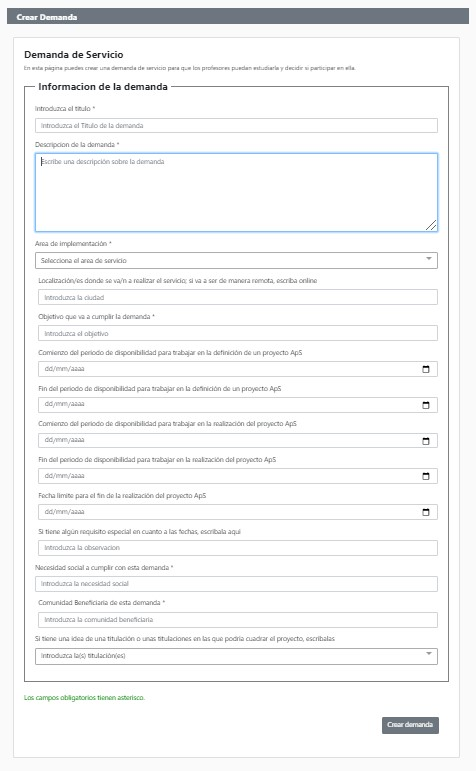
\includegraphics[scale=0.9]{demanda}
 	\caption{Formulario de creación de demanda}
 \end{figure}
 
 \section{Formulario creación oferta de servicio}
 Para poder crear una oferta de servicio es necesario crear el formulario de creación de una oferta de servicio. En el anterior TFG no existía este formulario, así que tuvimos que crearlo desde cero con sus correspondientes archivos para el correcto funcionamiento en Angular.\\\\
 Para el formulario de la creación de la oferta de servicio se han creado las validaciones correspondientes para los campos a completar, de manera que no se pueda permitir la creación de la oferta si alguno de ellos no está correcto y los mensajes correspondientes de error en este último caso. Los campos obligatorios tienen un asterisco y los opcionales no, tal como se puede observar en la figura \ref{fig:oferta}\\\\
 En función del campo se permiten los siguientes tipos de datos: \\
 \begin{itemize} 
 	\item En los campos \emph{título}, \emph{descripción}, \emph{asignatura/s objetivo}, \emph{observaciones temporales} se permite introducir texto.
 	\item En el campo \emph{año académico objetivo} se permite un valor de tipo numérico que represente un año válido.
 	\item El campo \emph{fecha límite} permite un valor de tipo fecha. Este campo es la fecha limite para terminar la definición del proyecto.
 	\item  El campo \emph{cuatrimestre objetivo} es un menú desplegable que permite una sola elección entre primer cuatrimestre, segundo cuatrimestre y anual. Si se selecciona un cuatrimestre sin seleccionar año académico, significa que el proyecto se desarrollara ese mismo cuatrimestre todos los años que dure el proyecto.
 	\item El campo \emph{Área/s de implementación} es un menú desplegable que permite selección múltiple. En el caso de que se haya seleccionado algún área de implementación por error se puede descartar la selección. Hay que seleccionar por lo menos una opción para que se pueda validar el campo correctamente.\\\\
 \end{itemize}
 Hemos comprobado los siguientes campos para poder validar el formulario correctamente:
 \begin{itemize} 
 	\item	El campo \emph{año académico objetivo} debe ser un año que no sea inferior al actual año.
 	\item	Si se especifica un año académico objetivo, la fecha límite para terminar la definición del proyecto y el año académico objetivo deben ser mayores que la fecha actual y menores que la fecha de comienzo del cuatrimestre especificado.\\\\
 \end{itemize}
 
 Consideramos como asignaturas TFM y TFG.
 Además, tuvimos que crear su correspondiente modelo con los campos necesarios para la creación de la oferta: identificador, titulo, descripción, imagen, fechas de creación y actualización, cuatrimestre objetivo, año académico, fecha límite, observaciones temporales, creador, área de implementación, asignatura (o asignaturas) objetivo y profesor ( o profesores). El creador es el profesor interno que está conectado en la aplicación y el cual accede a la creación de la oferta de servicio.\\\\
 
 
 \begin{figure}[t]
 	\centering
 	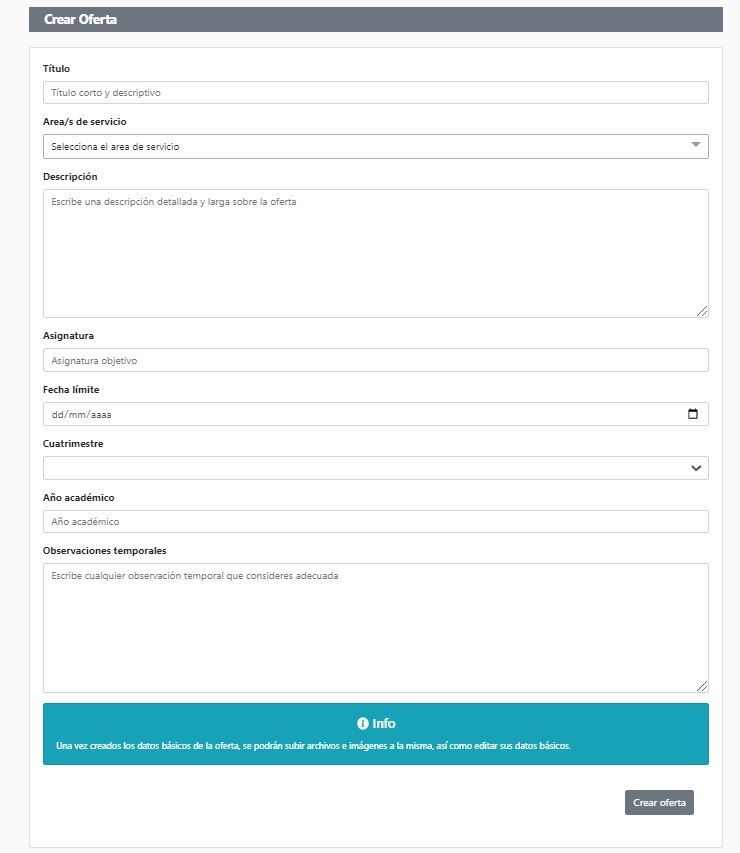
\includegraphics[scale=0.9]{oferta}
 	\caption{Formulario de creación de ofertas}
 \end{figure}
 \section{Formulario creación de partenariado profesor}
 Una vez creados los formularios de la oferta de servicio y la demanda de servicio, hemos procedido al desarrollo del formulario para la creación del partenariado por parte de un profesor.
 El formulario para la creación del partenariado no existía en el anterior TFG, así que se procedió a su creación desde cero. Para ello, tuvimos que crear los archivos y el modelo necesarios para el formulario. El formulario aparece con unos campos ya rellenos, algunos de los cuales son editables.\\\\
 En la creación del formulario de partenariado por parte del profesor, los datos de la demanda de servicio del socio comunitario beneficiario vienen ya completados y sin posibilidad de editarlos. Cuando un profesor interno respalda una demanda de servicio sin haber definido previamente una oferta de servicio, el formulario no viene con los datos de la oferta. Si la oferta de servicio existiera previamente, el formulario vendría con los datos ya rellenados.\\\\ 
 Hay dos maneras de crear un partenariado por parte de un profesor:
 \begin{itemize}
 	\item Un profesor interno comunica su intención de respaldar una
 	demanda de servicio que ha visto anunciada (y que ha sido creada
 	previamente por un socio comunitario).
 	El profesor rellena un formulario (no viene con datos de la oferta
 	porque no existe) y se crea un partenariado en estado \texttt{EN\_CREACION}.
 	A continuación, el socio comunitario rellena un formulario y el
 	partenariado pasa al estado \texttt{EN\_NEGOCIACION}.
 	\item Un profesor interno comunica su intención de respaldar una
 	demanda de servicio que le ha sido presentada como un match de una
 	oferta de servicio de la que es responsable. El profesor rellena un formulario (puede venir con datos tanto de la oferta como de la demanda) y se crea un partenariado en estado \texttt{EN\_CREACION}. A continuación, el socio comunitario rellena un formulario y el partenariado pasa al estado \texttt{EN\_NEGOCIACION}.\\\\
 	
 \end{itemize}
 El formulario está dividido en tres partes para la distinción entre los datos generales del partenariado que serán la combinación de los datos en común o los datos más relevantes del formulario, los datos de la oferta y los datos de la demanda. También hemos creado validaciones para todos los campos del formulario, para comprobar que tienen los datos validos en el formado apropiado para cada campo.\\\\
 En el formulario, el \emph{título} y la \emph{descripción } son una combinación de los \emph{títulos} y \emph{descripciones} de la oferta y la demanda. Estos campos son editables. Los datos de la demanda de servicio vienen rellenados, pero no son editables:  las \emph{áreas de implementación}, el \emph{socio comunitario} de la demanda, la \emph{localización de desarrollo} del partenariado, la \emph{finalidad}, la \emph{comunidad beneficiaria}, las \emph{observaciones temporales}, \emph{asignatura/s objetivo}, \emph{titulaciones tentativas}, \emph{cuatrimestre} y \emph{año académico}. Aparece como \emph{profesor responsable} el profesor de la oferta, siendo un campo editable que se da a elegir entre una lista de todos los profesores internos de la base de datos.\\\\
 El campo \emph{equipo de profesores} es una lista que da la posibilidad de selección múltiple y viene ya rellenada con los valores de la oferta de servicio ya creada, en el caso de que exista la oferta de servicio. El profesor que procede a la creación del formulario elige si se aceptan personas externas. El \emph{área de implementación} de la oferta no es un campo editable. Si algún dato no es completado adecuadamente, se mostrarán los mensajes para que informe al usuario de los campos a cambiar o completar. Si se valida el formulario, el estado pasa a \texttt{EN\_CREACION}. Si se rechaza pasa al estado \texttt{SUSPENDIDO}.
 \\\\
 
 
 \begin{figure}[t]
 	\centering
 	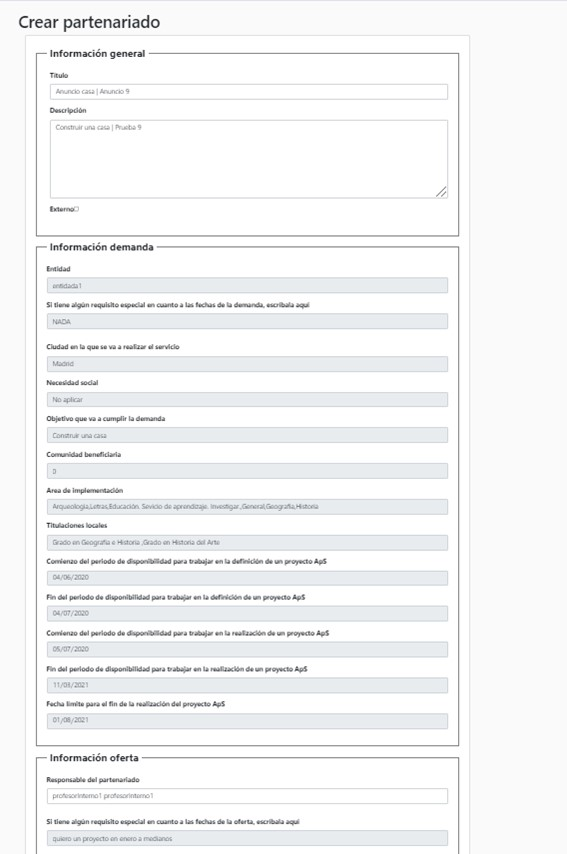
\includegraphics[scale=0.9]{partenariado1}
 	\caption{Formulario de creación de partenariado: parte 1}
 \end{figure}
 
 
 \begin{figure}[t]
 	\centering
 	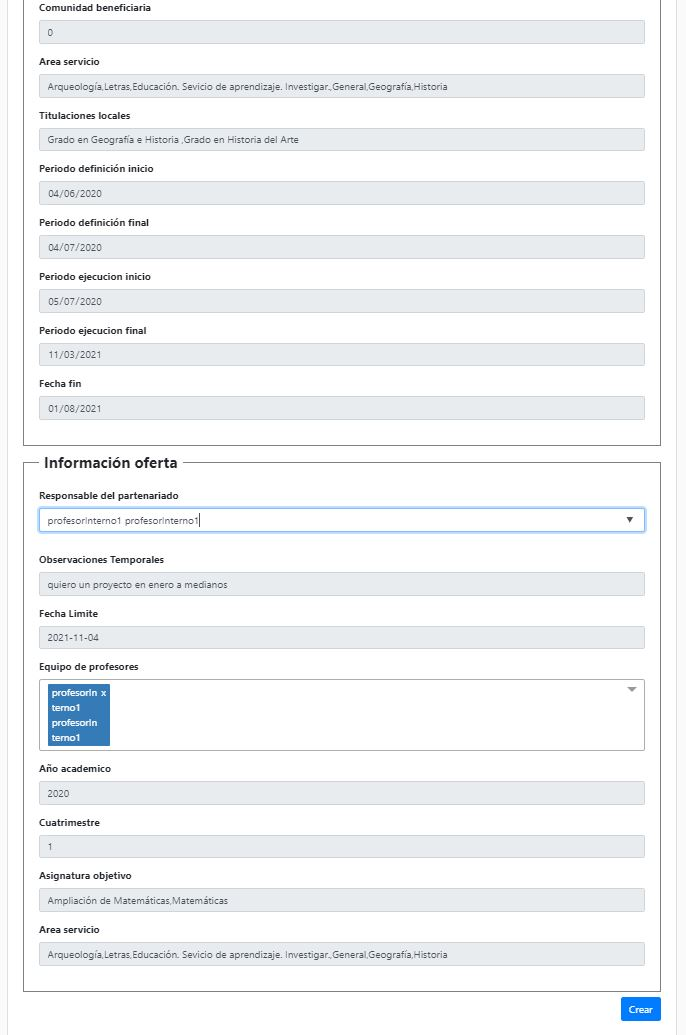
\includegraphics[scale=0.9]{partenariado2}
 	\caption{Formulario de creación de partenariado: parte 2}
 \end{figure}

\chapter{Contribución}
A continuación, se detallan las contribuciones de cada uno de los componentes del grupo ordenados por orden alfabético.
\section{Daniela-Nicoleta Boldureanu}
La primera fase consistió en investigar, tarea que fue realizada por todos los miembros del TFG.\\
En la segunda fase del proyecto Daniela se ha encargado de arreglar \textit{bugs} del trabajo anterior, tales como:
\begin{itemize} 
	\item Hacer que las contraseñas sean robustas y que el usuario no pueda registrarse con una contraseña que tenga menos de ocho dígitos, que no contenga ninguna mayúscula, minúscula o carácter especial. Además, arregló el mensaje de error de la contraseña defectuosa porque saltaba siempre cuando otro campo del formulario estaba mal.
	\item Comprobar que los campos \emph{contraseña} y \emph{repetir contraseña} del registro y editar perfil usuario sean iguales y mostrar el correspondiente mensaje al validar ambos formularios.
	\item Si se introducía un correo incorrecto no saltaba ningún mensaje de error.
	\item Corregir faltas de ortografía o palabras repetidas en algunas páginas de la aplicación.
	\item En el perfil del socio comunitario en la página para editar una iniciativa, proyecto o partenariado al subir un fichero o una foto, si luego se borraba y se intentaba subir de nuevo el mismo fichero/foto, no se subía.
	\item En el perfil del estudiante en la página de editar perfil si se subía una foto, se borraba y luego se volvía a subir la misma imagen, no se subía.
\end{itemize}

En la tercera fase del TFG Daniela se ha encargado de empezar el modelo de dominio y el modelo de datos usando Modelio. En paralelo ha creado las tablas \textbf{estudiante, estudiante\_externo, estudiante\_interno, usuario, oficina ApS, Admin, entidad, profesor-colaboración, profesor y profesor\_interno} en la base de datos. También unificó todas las tablas de la base de datos una vez creadas. El proceso de unificar consistió en hacer que todos los nombres estén en el mismo formato, qué todos los atributos tengan el mismo cotejamiento, qué atributos del mismo tipo tengan la misma longitud y que los enumerados tengan el mismo formato. Con crear las tablas nos referimos a crear la estructura, definiendo los nombres de los campos y los tipos de datos, y creando restricciones entre las tablas.\\\\
En la cuarta fase Daniela se ha encargado de desarrollar el DAO llamado \textit{Usuario} que implementa el acceso a la base de datos del grupo de tablas llamado \textit{Usuario} que se puede ver en la Figura \ref{fig:usuarios}. La creación de este DAO ha supuesto la necesidad de la creación de diez \textit{transfers} que alojan los datos del elemento Usuario, Estudiante, Estudiante Externo, Estudiante Interno, Profesor, Profesor Externo, Profesor Interno, Entidad (socio comunitario), Oficina ApS y Admin . Los DAOs han sido implementados usando Knex.js, una librería que facilita las consultas a la base de datos. En el DAO \textit{Usuario} se crearon las funciones CRUD de Usuario, Estudiante, Estudiante Externo, Estudiante Interno, Profesor, Profesor Externo, Profesor Interno, Entidad (socio comunitario), Oficina ApS y Admin. Todos están relacionados uno con el otro. También se creó el método para obtener todos los datos de los profesores internos en función de una estructura de datos que recibe como parámetro y que contiene los identificadores de unos profesores internos.\\
Después de finalizar la implementación del DAO \textit{Usuario} Daniela desarrolló los métodos CRUD del elemento \textit{Proyecto} perteneciente al DAO \textit{Colaboración}. Este DAO implementa las tablas pertenecientes al grupo \textit{Colaboración} que se puede ver en esta Figura \ref{fig:colaboracion}. Además, fue necesario crear un transfer \texttt{Notas} y desarrollar los métodos CRUD del elemento \textit{Nota}.\\
 Daniela implementó en el DAO \textit{Usuarios} cuatro métodos para obtener las titulaciones locales de un profesor interno en función de su identificador, obtener todas las universidades, obtener todas las titulaciones locales y obtener todas las áreas de implementación de la base de datos. Estos cuatro métodos han servido para el registro de usuario, la creación de la oferta, la creación de la demanda y del partenariado por el profesor.\\
  Además, ha creado los siguentes scripts necesarios para insertar los valores de los enumerados con Python:
\begin{itemize} 
	\item Recoger las universidades de una hoja de cálculo Excel, procesar los valores y añadirlos en la tabla \texttt{universidad} de la base de datos.
	\item Recoger las titulaciones locales de una hoja de cálculo Excel, procesar los valores y añadirlos en la tabla \texttt{titulación\_local} de la base de datos.
	\item Recoger las áreas de conocimiento de una hoja de cálculo Excel, procesar los valores y añadirlos en la tabla \texttt{área\_conocimiento} de la base de datos.
	\item Recoger las áreas de implementación de una hoja de cálculo Excel, procesar los valores y añadirlos en la tabla \texttt{área\_servicio} de la base de datos.\\\\
	\item Recoger las necesidades sociales de una hoja de cálculo Excel, procesar los valores y añadirlos en la tabla \texttt{necesidad\_social} de la base de datos.\\\\
\end{itemize}
En la quinta fase Daniela se ha encargado de adaptar el código de obtener los datos de la página principal y de crear los correspondientes métodos en el DAO Colaboración: obtener el número de proyectos, el número de partenariados y el número de iniciativas existentes en la base de datos.\\ 
También se ha encargado de crear los métodos del \emph{matching} para obtener las coincidencias en las observaciones temporales de la oferta de servicio y de la demanda de servicio y de obtener las coincidencias de las descripciones tanto de la oferta como de la demanda de servicio mediante Procesamiento del Lenguaje Natural (NLP). Para realizar este procesamiento adecuadamente fue necesario investigar sobre las herramientas disponibles. Para ello tuvo que buscar la lista de todas las palabras vacías del idioma español. Una vez acabada la investigación y encontradas las palabras vacías, desarrolló el algoritmo.\\\\
En la quinta fase Daniela se ha encargado de adaptar, añadir nuevos campos y crear los mensajes correspondientes para los formularios de registro y editar usuarios. Adaptó la aplicación tanto de \textit{front-end} como de \textit{back-end} en la parte de usuarios y página principal. Este proceso fue complejo dado que requería mucho conocimiento tanto en Angular como en NodeJS y fue un paso importante para la creación de los formularios de la oferta, de la demanda y del partenariado por parte del profesor. También ha desarrollado la parte de \textit{front-end} del formulario para crear el partenariado por parte del profesor.

\end{document}
